\documentclass{ar2rc}

\usepackage{graphicx}
\usepackage{beraserif}
\usepackage{natbib}
\usepackage{color}


\title{An Improved Minimum-Distance Texture Estimator for Speckled Data under the $\mathcal{G}^0$ Model}
\author{Julia~Cassetti,
	Alejandro~C.~Frery}
\journal{Journal of Mathematical Imaging and Vision}
%\doi{12345}

\begin{document}
	
	\maketitle
	
	\section{Reviewer \#1}
	
	\subsection{Summary}
	
\fbox{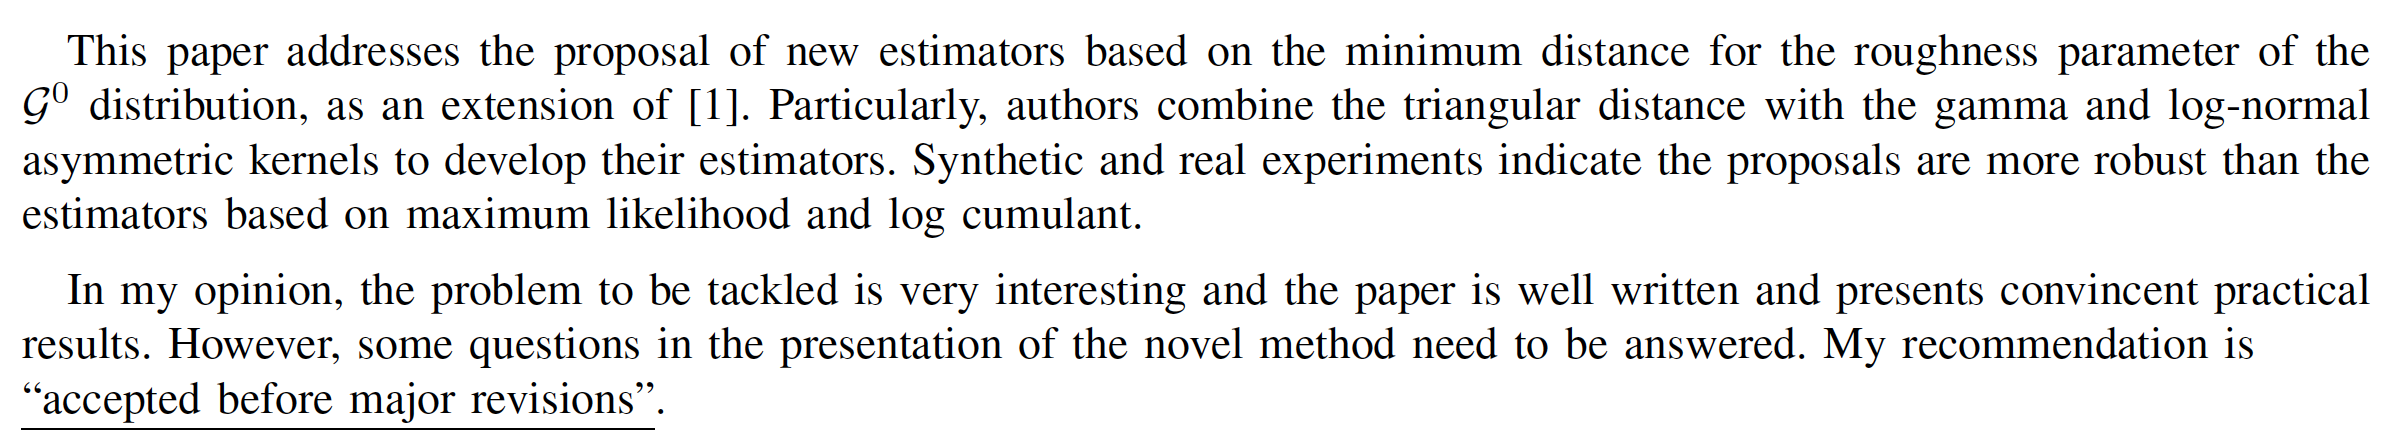
\includegraphics[width=\linewidth]{Summary}}	

\AR We would like to thank the reviewer for the careful analysis of our work.
We agree with the suggestions, and we have proceeded accordingly.
	
	\subsection{Critical comments}

\fbox{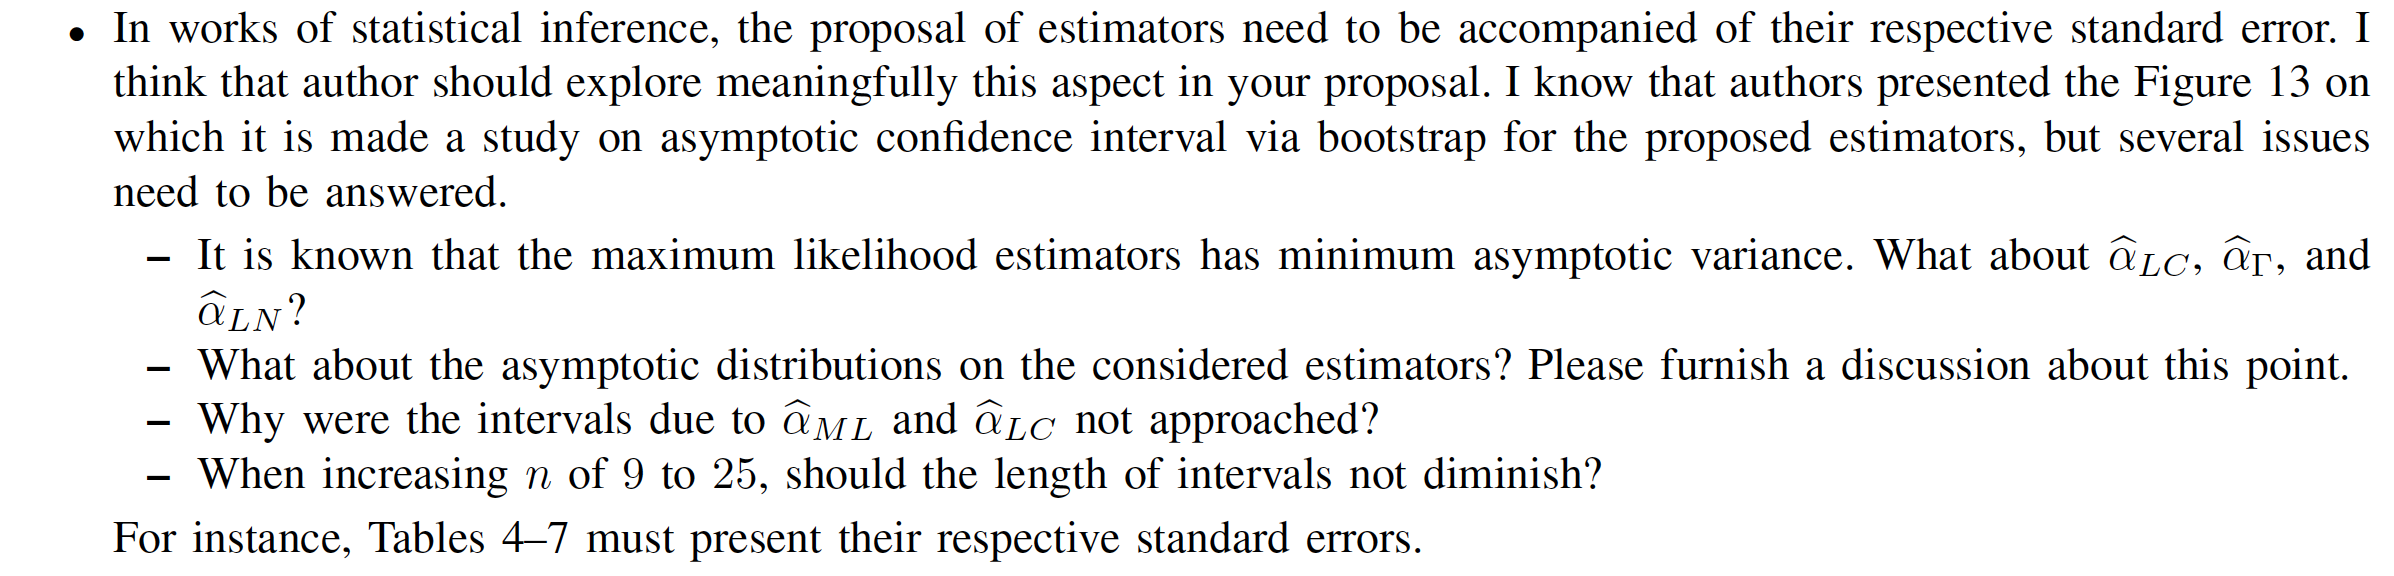
\includegraphics[width=\linewidth]{Critical}}

\begin{itemize}
	\item [-] \textcolor{blue}{We added Table 5 and its corresponding analysis.}
	
	\item [-] \textcolor{blue}{We include Fig. $5$ and $6$. The former displays the distribution of estimators for $\alpha=-3$, $L=3$ and for different sample sizes including $n=500$. The latter exibit the density function for different values of the texture parameter, and for a sample size equal to $500$. We also present the values of skewness, kurtosis in Table $4$ and $5$ respectively. It is accompanied by an analysis of the figures and tables.}
	
	\item [-] \textcolor{blue}{Thank for your observation. There was an error in Fig. $15$. We fixed this error and also add Table $11$ which shows the length of the bootstrap confidence intervals.}
	
	\item [-] \textcolor{blue}{It can be seen in Table $11$ that the length of the confidence intervals decrease as the sample size increases.} 
	For instance, Tables 4-7 must present their respective standard errors.
	\textcolor{blue}{Falta esto útlimo}
\end{itemize}




\subsection{Detailed comments}

\fbox{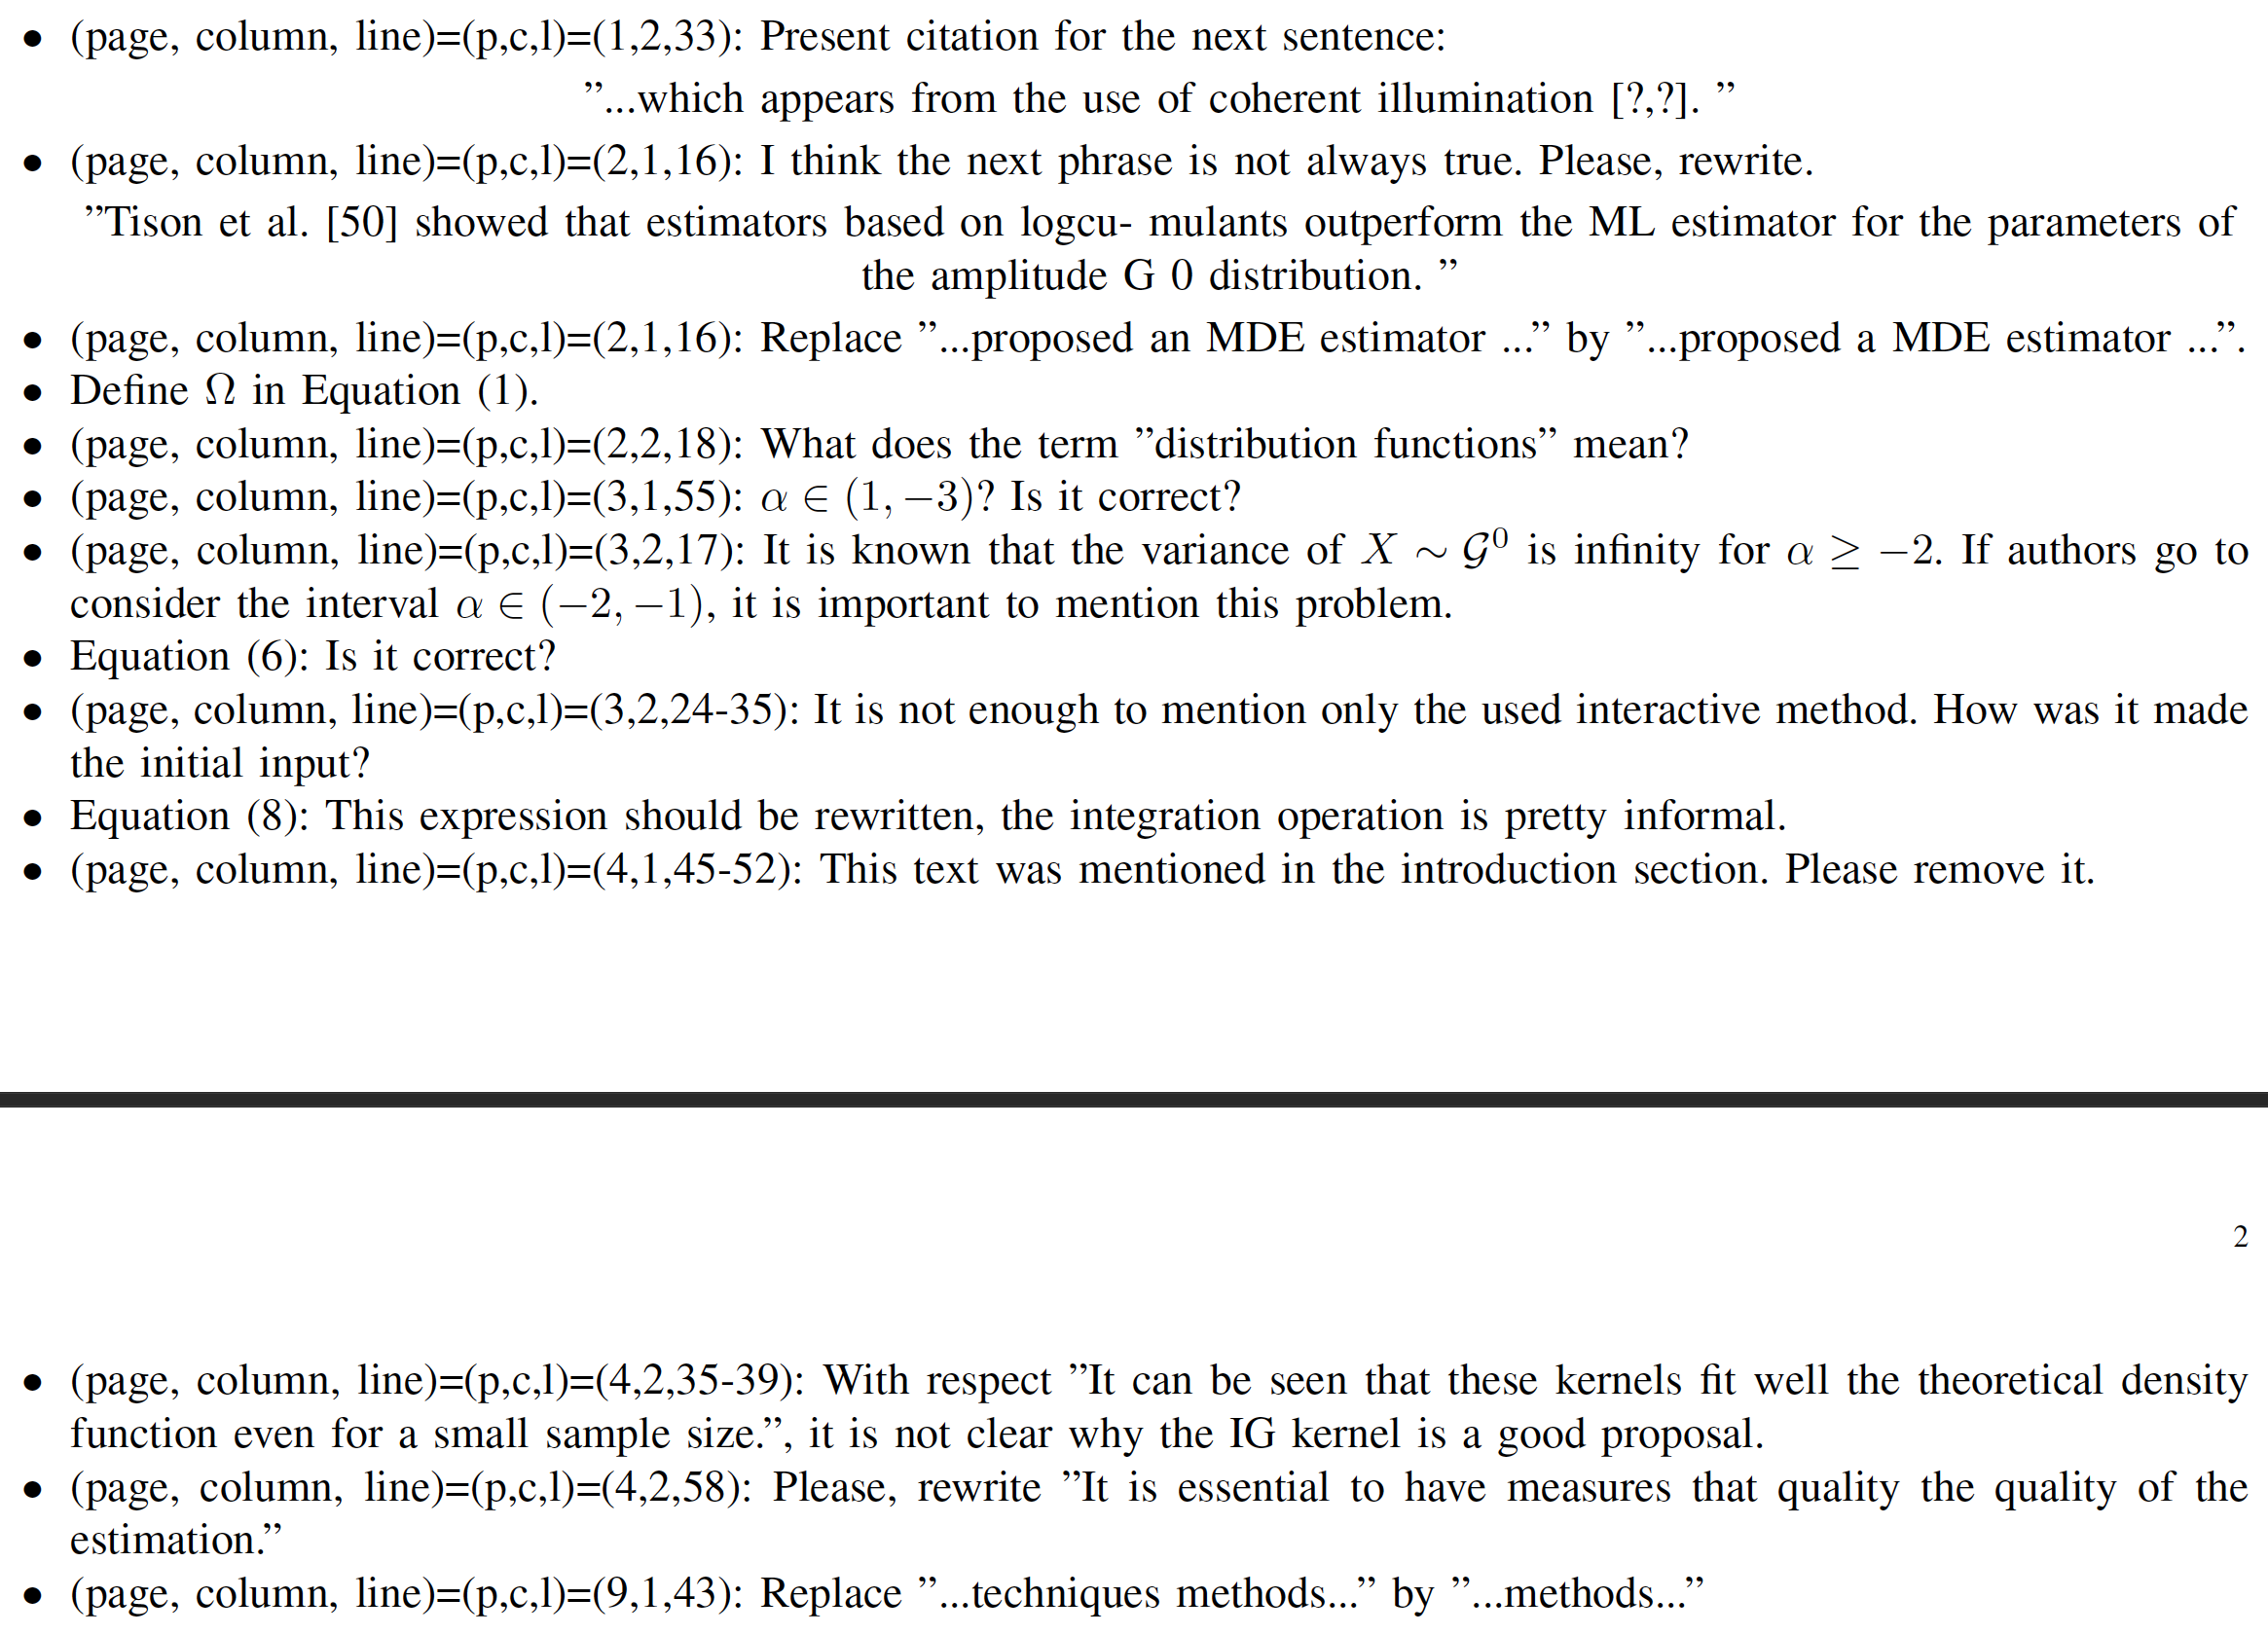
\includegraphics[width=\linewidth]{Detailed}}

\AR We have made the following changes:
\begin{itemize}
\item We have added the reference by \citet{SARImageStatisticalModelingPartISinglePixelStatisticalModels}, which is a modern and comprehensive survey about speckle.
\item 
\item 
\item We added ``and $\Omega$ is the parameter space.'' to the sentence after~(1).
\item We changed the text as follows:
		\begin{quote}
	In particular, several measures have been proposed to reflect the closeness  \DIFdelbegin \DIFdel{between two distribution functions.} \DIFdelend \DIFaddbegin \DIFadd{among the models that describe samples.}\DIFaddend
		\end{quote}
\item It was wrong; we corrected it and now it reads \textcolor{blue}{``$\alpha \in (-3,-1)$''}.
\item \textcolor{blue}{Falta, creo que me dijiste que te la deje}
\item The equation $6$ is correct. We only consider the terms that depend on $\alpha$, which are those involved in the minimization.
\item We added the following text to explain which was the initial point that was considered in the algorithm.
\begin{quote}
	taking as a starting point $\alpha_0$ the alpha moment estimator when it exists. Otherwise we consider $\alpha_0=-1.5$.
\end{quote}
\item We rewrite equation $8$ as 
\begin{equation}
	d_{\text{\tiny{T}}}(f_{\text{\tiny{V}}},f_{\text{\tiny{W}}})=\int_{S}\frac{(f_{\text{\tiny{V}}}(x)-f_{\text{\tiny{W}}}(x))^2}{f_{\text{\tiny{V}}}(x)+f_{\text{\tiny{W}}}(x)}dx,
	\label{DT}
\end{equation}

\item Following your request this paragraph was deleted.
\item We explain this in the text as follows:
\begin{quote}
	It can be seen that these kernels fit reasonably well the theoretical density function even for a small sample size. The IG kernel presents a good approximation to the true density function at the center of the function although heavier tails are observed. The $\Gamma$ and LN kernels show a better fit, with the latter kernel having a higher kurtosis than the other kernels.
\end{quote}
\item We changed the text as follows:
	\begin{quote}		
	It is essential to have measures that \DIFdelbegin \DIFdel{quality} \DIFdelend \DIFaddbegin \DIFadd{quantify }\DIFaddend the quality of the estimation. 
	\end{quote}
\item We deleted the word ``techniques''.
\end{itemize}

\bibliographystyle{agsm}
\bibliography{../../../../../Bibliography/bib_julia2}
	
\end{document}
